\noindent
Di seguito vengono spiegati l'utilizzo degli strumenti di modifica delle presentazioni.

\subsection{Menù laterale}
\begin{itemize}
 \item \textbf{Text}\\
    Premendo il pulsante del menù laterale \textbf{Text} verrà aggiunto alla slide corrente un campo di testo.
    \begin{figure}[h] 
	\centering 
	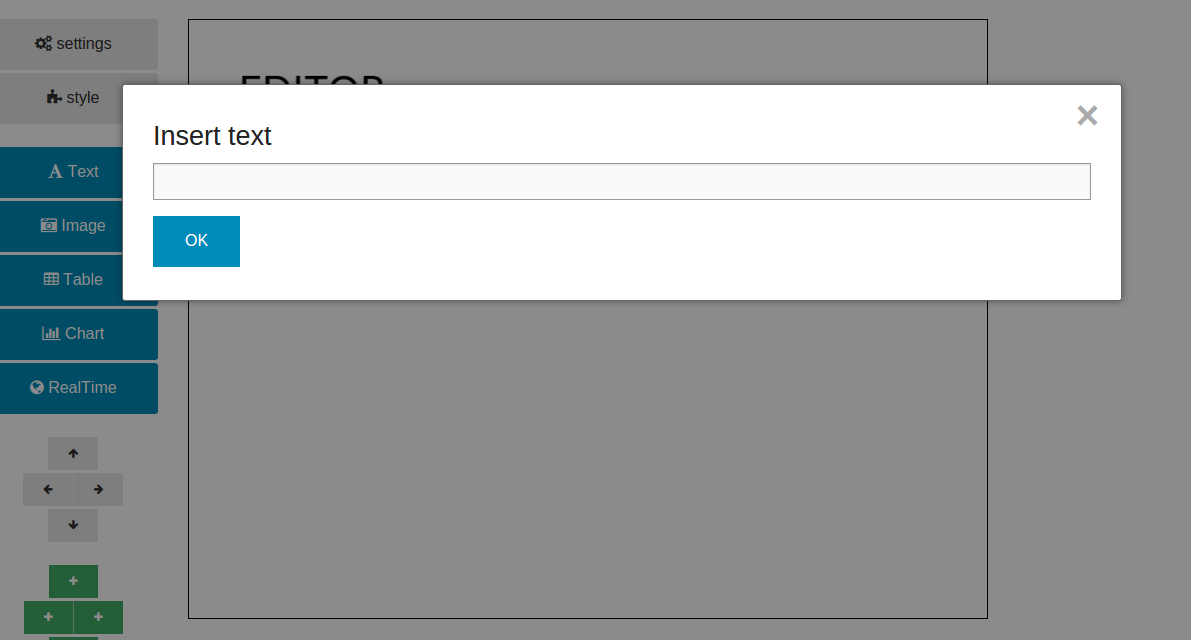
\includegraphics[scale=0.30] {img/MUAddText.png}
	\caption{Slide Editor - Aggiunta testo} 
    \end{figure}
 \item \textbf{Image}\\
    Premendo il pulsante del menù laterale \textbf{Image} verrà visualizzata una finestra che permette di aggiungere un'immagine alla slide corrente tra quelle già caricate o di caricarne un'altra.
     \begin{figure}[h] 
	\centering 
	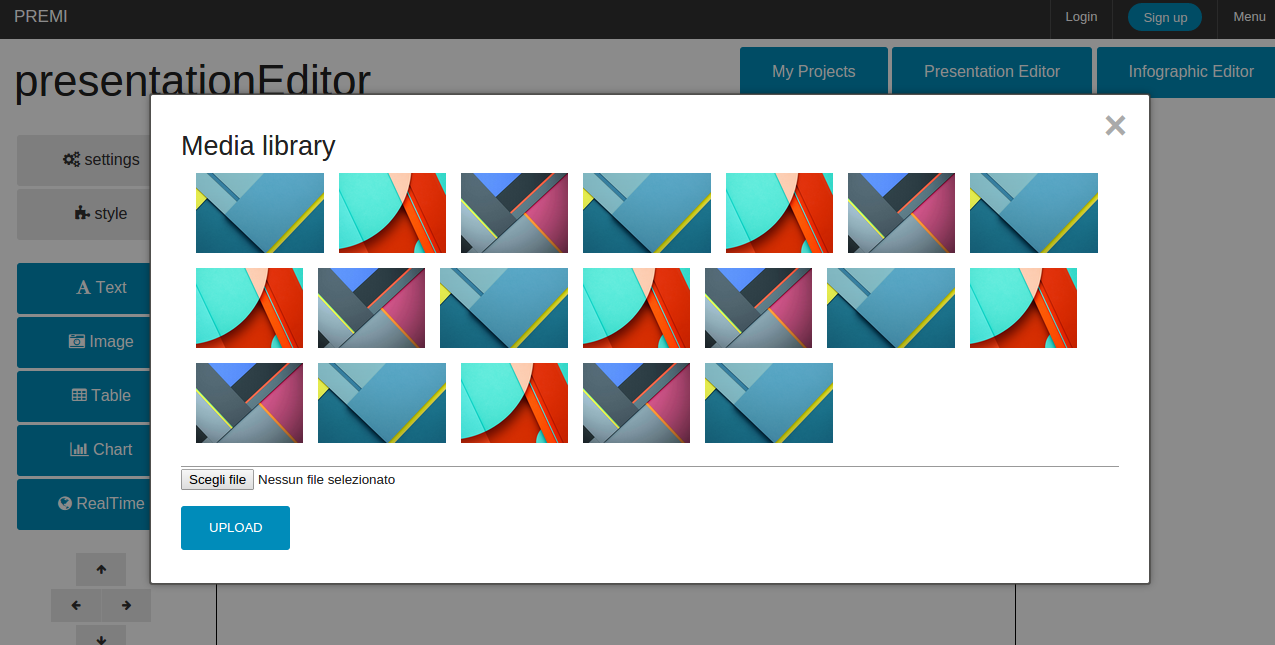
\includegraphics[scale=0.30] {img/MUAddImage.png}
	\caption{Slide Editor - Aggiunta immagine} 
    \end{figure}
 \item \textbf{Table}\\
    Premendo il pulsante del menù laterale \textbf{Table} verrà aggiunta una tabella alla slide corrente.
 \item \textbf{Chart}\\
    Premendo il pulsante del menù laterale \textbf{Chart} verrà aggiunto un grafico alla slide corrente.
 \item \textbf{RealTimeData}\\
    Premendo il pulsante del menù laterale \textbf{RealTimeData} verrà aggiunto componente rappresentante i valori, presi in tempo reale, con un formato adeguato.
\end{itemize}


\subsubsection{Style}
Premendo il pulsante del menù laterale \textbf{Style} verrà visualizzata una finestra nella quale si potrà scegliere il colore della slide e l'effetto di transizione.
\subsubsection{Settings}
Premendo il pulsante del menù laterale \textbf{Settings} verrà visualizzata una finestra nella quale si possono modificare le opzioni generali della presentazione.

\subsection{Modifica di un componente}
Per modificare un componente è sufficiente selezionarlo nella slide e modificarne gli attributi dal menù che comparirà sulla destra.
\begin{itemize}

	\item \textbf{Text:}
		\begin{itemize}
			\item Dimensione font;
			\item Tipo di font;
			\item Dimensione campo di testo;
			\item Rotazione;
			\item Allineamento.
		\end{itemize}
		 \begin{figure}[h] 
		    \centering 
		    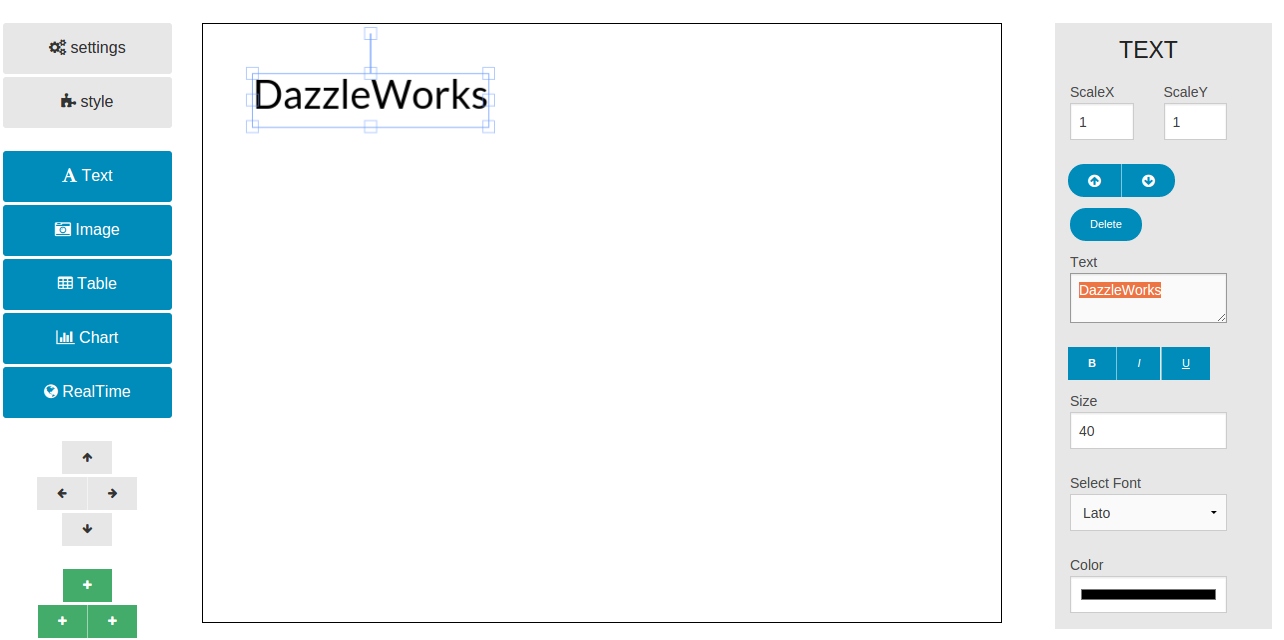
\includegraphics[scale=0.37] {img/MUslideEditor.png}
		    \caption{Slide Editor - Modifica testo} 
		\end{figure}
	
	\item \textbf{Image:}
		\begin{itemize}
			\item Dimensione;
			\item Colore di sfondo;
			\item Opacità;
			\item Rotazione.
		\end{itemize}

	\item \textbf{Table:}
		\begin{itemize}
			\item Numero di colonne;
			\item Numero di righe;
			\item Dimensione;
			\item Rotazione;
			\item Colore di sfondo.
		\end{itemize}
		
	\item \textbf{Chart:}
		\begin{itemize}
			\item Dimensione;
			\item Tipo di grafico;
			\item Dati;
			\item Rotazione;
			\item Colore di sfondo.
		\end{itemize}
	
	\item \textbf{RealTimeData:}
		\begin{itemize}
			\item Dimensione;
			\item Rotazione;
			\item Indirizzo;
			\item Tipo di dati;
		\end{itemize}
\end{itemize}

\noindent Per modificare la dimensione di un componente è anche possibile selezionarlo e trascinare i bordi e gli angoli del riquadro direttamente nella schermata che mostra gli elementi inseriti nella slide. Il trascinamento in un angolo provoca una variazine della dimensione proporzionale tra larghezza ed altezza. 
 
\subsection{Aggiunta di una slide}
Per aggiungere una slide a destra o in basso è sufficiente premere il simbolo \textbf{+} corrispondente nella direzione desiderata.
\begin{figure}[h] 
      \centering 
      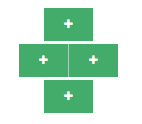
\includegraphics[scale=0.37] {img/piu.png}
      \caption{Slide Editor - Modifica testo} 
  \end{figure}
\subsection{Navigazione delle slide}
Per navigare tra una slide e l'altra bisogna utilizzare i tasti freccia situati sotto a quelli per l'aggiunta di una slide.
\begin{figure}[h] 
		    \centering 
		    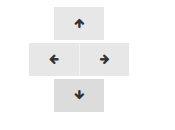
\includegraphics[scale=0.37] {img/frecce.png}
		    \caption{Slide Editor - Modifica testo} 
		\end{figure}